\chapter{Introduction}

% In this chapter, we introduce the fundamentals of genetics and DNA sequencing. Furthermore, we introduce the important research problem in the field of genetics, the diploid genome assembly (haplotyping). 
% We will see how we can mathematically formualate the diploid assembly problem as a computer scientist.
% Then we provide a high level description of the main methods used in this problem.
% Thereafter, we describe the limits and challenges faced currently in this field. We finish this chapter by an outline of the thesis.


Genetics studies the incredible phenomenon of \textit{life} at its most basic level, thus the science of genetics is tremendously important and fascinating.
% In this section we describe the basics about genetics and haplotyping. We provide motivation about why understanding genetics for different organisms is so important.
% https://www.gen.cam.ac.uk/undergraduate/whygenetics
% http://www.helsinki.fi/biosciences/genetics/
An important field in genetics is haplotyping.
Haplotyping is the process of determining the sequences of both homologous copies, which are inherited from each parent in diploid organisms.
It has applications in different fields such as evolutionary studies, clinical diagnosis, precision medicine, and biotechnology. 
Current sequencing technologies allow us to read this genetic code, and thus the reconstruction of haplotypes is
possible. Unfortunately, sequencing is prone to error and the use of advanced algorithms and models are essential to alleviate these errors, in order to reconstruct accurate haplotypes.  
In this thesis, we study how we can address different computational challenges in this field using clever algorithms.

\section{Genetics, DNA sequencing and Haplotyping}
Genetics is the study of genes, genetic variation, and heredity in living organisms. 
Genetics controls what an organism looks like and how it functions.
% The DNA is the carrier of hereditary information and thus understanding DNA in detail has been the central aim for many researchers.
% Classically the genetic variants (mutations) present in the living organisms have been used to study and investigate the cause of biological diseases and, additionally helps to make deductions about the way cells and organisms worked. 
% Genetics is the study of genes, genetic variation, and heredity in living organisms.
Classically, there are two sides to the science of genetics.
On one side, the availability of different types of molecular information, such as sequence information and gene expression, paired with gene editing techniques, 
provides powerful explanation about the functions of the genes.
On the other side, genetics provides a fundamental understanding of how organisms, populations, and species evolve. 
In the last few years, one of the most exciting new developments, is the way in which these two sides have begun to converge.
This is achieved through the integrative effort of using molecular techniques to understand development, evolution, and speciation.
Modern computational biology tools (analysis of genomic sequences and bioinformatics) use these integrative principles 
to answer some difficult biological questions ranging from evolution to complex diseases.
Thus, genetics has a central role in modern biology and its influence is ever increasing.

% s\todo{citations are missing in this para or even figures.}
% from italy person thesis.
\textit{What actually is genetic information?} 
The discovery of double helix deoxyribonucleic acid (DNA) by Watson and Crick in 1953, laid the main foundation for the understanding of genetics.
In most living organisms, genetic information is encoded in the form of DNA molecules.
A DNA molecule is a chain in which many bases are ordered in a linear sequence, the bases --- A, T, G, and C --- are the letters of the genetic alphabet.
The whole information within the DNA molecule of an organism is called its genome. The genome is further divided into chromosomes.
Genomes have single (haploid), double (diploid) or higher ploidy (polyploids). 
In this study, we focus on \textit{diploid} organisms. For example, humans are diploids, consisting of two copies of each chromosome called homologous chromosomes or \textit{haplotypes} --- one inherited from the mother and the other from the father.
There are differences between these two copies of each chromosome known as genetic variation. 
% \todo{this para explained in more detail in biological background.}

In 2001, a historic breakthrough happened with the sequencing of the human genome \citep{collins2003human}.
\textit{Sequencing} is the operation that comprises in determining the base sequence of a DNA molecule.
For sequencing genomes, there exist several kinds of sequencing technologies which share the following common properties:
\begin{itemize}
 \item They yield genomes in fragments or pieces called ``reads''.
 \item The position of reads is unknown over the genome and also, most of the times, the strand from which the read was sampled is unknown.
 \item The reads contain errors.
\end{itemize}

Huge amounts of sequencing data are produced by next generation sequencing technologies (NGS) routinely. 
The major challenge with these sequencing datasets is that the genomic information is partial and erroneous. Therefore, no sequencing technology delivers the completely sequenced genome.

The major differences between these technologies are error rates and the read-lengths. We define the error rate of a read as the ratio of the number of incorrectly sequenced bases to the length of the read.
Broadly, the sequencing technologies can be categorized into four classes:
\begin{itemize}
 \item Short read sequencing: It includes Illumina/Solexa sequencing \citep{bentley2008accurate}, which has been the most widespread technology. 
 It produces shorter reads (hundreds of bases) with high accuracy ($\le 1$\%). 
  \item Long read sequencing: It includes Single Molecule Real Time sequencing (PacBio) \citep{eid2009real} and Oxford Nanopore sequencing (ONT)\citep{laszlo2014decoding}. They produce very long sequences, up to hundreds of kilo-bases. 
  The downside is that PacBio and ONT exhibit very high error rates of up to 15\% and 38\% respectively. 
  \item Synthetic long read sequencing: It includes 10x Genomics technology \citep{eisenstein2015startups}, which produces synthetic long reads and relies on short-read Illumina platform.
 \item Single-cell sequencing: It includes Strand specific sequencing (Strand-Seq), which produces Illumina reads, along with directionality of DNA. Each single strand of a DNA molecule is distinguished based on its 5'–3' orientation \citep{falconer2012dna}.
\end{itemize}

Furthermore, each sequencing technology has some bias due to the protocols employed.
The high G/C content regions are less covered by the short read technologies and the read ends present high error rate \citep{aird2011analyzing, dohm2008substantial}.
Taken together, each sequencing technology comes with its own advantages and disadvantages, which indicates that the potential way of generating complete genomes could be to integrate all the information available from different sequencing technologies.

\textit{What are the obstacles across all technologies in producing a diploid genome?}
For all the existing sequencing technologies, the first challenge comes from the lack of information of the \textit{genomic origin} of reads.
For diploid organisms, the next challenge is the lack of the \textit{haplotypic identity} of reads, meaning, the haplotype that the read comes from.
Reconstructing both copies of each chromosome is necessary to understand the true characteristics of diploid organisms.
% Thus, from the biological point of view, the single individual haplotyping (SIH) problem consists in the reassignment of each read to the original haplotype.
% Once we know this identity, it becomes easier to assemble the reads from each haplotype separately to further reconstruct the two genome sequences of diploid organisms.
% The process of reconstructing the diploid assemblies from sequencing reads is known as \textit{diploid genome assembly} or \textit{haplotyping}.

These haplotypes are required in order to correctly understand allele-specific expression and compound heterozygosity, also investigating the genetics of common diseases, and to performing population genetic analyses of admixture, migration and selection \citep{tewhey2011importance, Glusman2014}. 
Furthermore, these haplotype sequences are used in relating genotypes to phenotypes and for understanding how the arrangement of cis- and trans-acting variants across the two homologous copies of a genomic region affects phenotypic expression.

\begin{figure}[t!]\centering
\includegraphics[width=\columnwidth]{{ex1-intro1}.pdf}
\caption{Seven variants covered by reads (horizontal bars) in a single individual.
The alleles that a read supports are printed in white. The middle panel shows the phased reads in colors and haplotypes at the bottom over the seven variants.}
\label{fig:ex1_intro}
\end{figure}

Broadly, the approaches to obtain haplotypes are classified into two categories:
\begin{itemize}
 \item Reference-based haplotyping
 \item \textit{de novo} assembly
\end{itemize}

% This absence of context and the small size and error rates of the sequences obtained, relatively to the genome size, makes it difficult to use reads as such.
% Ideally, we would need the access to the underlying genomes in their entirety.
% Since the beginning of sequencing of DNA molecules, genomes are produced by structuring and ordering reads information. 
% Then these reconstructed genomes can be used
% as references. 
Reference genomes are a reliable source to know the genomic origin of reads. 
Over the years, a lot of efforts have been devoted to generate good quality reference genomes.
Together with the gene sequences information that lead to proteins, the reference genomes also play an important role in gene regulation of living beings \citep{encode2004encode}. 
They also reveal the inner organization of the genome,
including the relative positions of genes or chromosomes structure. 
They have been used by biologists for other tasks, for instance, finding about the known genes
positions and functions to annotate the genome \citep{harrow2012gencode}.

Therefore, the reference genome is a good reference to solve the problem of identifying the origin of each read, sequencing reads have been aligned to the reference genome, which provides potential ordering of reads.
Once the reads are aligned to the reference genome, the aligned reads are then partitioned to two sets to generate haplotypes. This process is called \textit{reference-based} haplotyping (phasing).

In reference-based haplotyping, there is a reference bias attached to it. To overcome this problem, this approach is generalized to perform \textit{haplotype-aware} de novo assembly.
In this approach, the reference genome is not used, the haplotypes are instead constructed directly from the reads.
% In a reference-based approach, the reads are aligned to the reference genome and then the aligned reads are partitioned into two sets to generate the haplotypes.
% This process is 
% To determine the assignment of each read to one of the homologous copies of chromosome (haplotype) is an important question. 
% Thus, from the biological point of view, the haplotyping (SIH) problem consists in the reassignment of each read to the original haplotype.
% Once we know this identity, it becomes easier to assemble the reads from each haplotype separately to further reconstruct the two genome sequences of diploid organisms.
% The process of reconstructing the diploid assemblies from sequencing reads is known as \textit{diploid genome assembly} or \textit{haplotyping}.
First, we present formulation and methods to solve reference-based haplotyping (single individual haplotyping) and then generalize them to perform \textit{haplotype-aware} de novo assembly.
\section{Reference-based Haplotyping}
The \textit{reference-based} phasing method is used when we already have a reference for the species of the individual sequenced.
We expect the target genome to be very close to the reference, more specifically, we expect the reference to be from the same species as the reads. We are interested to phase the differences of target genome to its reference.
The usual pipeline for reference-based phasing consists of the following steps: 
\begin{itemize}
 \item Align the reads to the reference genome.
 \item Detect variants based on aligned reads.
 \item Phase the variants using the aligned reads.
\end{itemize}
The main focus of this study is on the third point in the pipeline.
% For illustration, the toy example is given in Figure~\ref{fig:ex1_intro}.

\begin{example}
 To illustrate the haplotyping problem for a single genome, we consider a small example in Figure~\ref{fig:ex1_intro}. The example shows seven variants. Also shown are the sequencing reads aligned to the reference genome.
 The alleles that a read supports are printed in white. 
 The sequencing reads contain erroneous alleles are shown in red. The goal of \textit{reference-based} haplotyping problem is the re-assignment of phases to the reads. 
 It is shown in the middle panel with the colored bars representing the assignment of each read to green or purple haplotype.
 Finally, the reads from each haplotype are separately assembled together to output two haplotypes shown at the bottom in purple and green.
\end{example}
\begin{figure}[t!]\centering
\includegraphics[width=\columnwidth]{{ex1-intro}.pdf}
\caption{Example shows the SNP matrix for the example shown in Fig.~\ref{fig:ex1_intro}. Seven variants covered by reads (horizontal bars) in a single individual.
 The allele in read is encoded as 1 if it matches the allele in the reference position at that position.
 The middle panel shows the phased reads in colors and haplotypes at the bottom over the seven variants.}
\label{fig:ex1_intro1}
\end{figure}

% you may refer also this: http://homolog.us/Tutorials/index.php?p=1.4&s=1

\subsection{Haplotyping as Combinatorial Optimization problem}
Large volume of sequencing data, which contain errors, is generated every day and extracting useful information from these datasets to understand the biology of diploid genomes is a challenging problem. 

The study of how to solve problems to achieve the best possible goal, or objective, has created the field of \textit{optimization}.
An \textit{optimization} problem is defined as: given an object $\mathfrak{x}$, find a solution such that an optimization criterion $\mathfrak{f}$ is minimized or maximized.

% Reference genome reconstruction is therefore crucial in various domains where raw,
% out of context reads are unusable. The task of reordering the reads to reconstruct the
% sequenced genome for diploid organisms is called diploid genome assembly or haplotyping.
% Over the genome, there are difference between two copes for each chromosome, known as variants \todo{explained in biological background}. 
% Traditionally, there are two ways to solve it, one is based on the ordered reads to the reference genome and the other one is \textit{denovo assembly}.
% As it will be detailed further, diploid genome assembly is especially complex as the bases distribution is far
% from being uniform. Genomes present specific patterns such as large repeated sequences
% (repeats), regions with very specific distributions of nucleotides or extremely repeated
% sequences of nucleotides. Such patterns make genomes different from a uniformly distributed sequence of nucleotides. \todo{[13]} shows that a human genome is largely constituted
% of repeated sequences of significant lengths.


% \fbox{\begin{minipage}{30em}
%  In summary, the core messages of DNA, sequencing and haplotyping:
%  \begin{itemize}
%   \item The molecular information of the genomes can be obtained using different sequencing technologies.
%   \item The sequencing data is big, erroneous and not complete.
%   \item The task of recovering the genome sequences for diploid organisms is called as diploid genome assembly or haplotyping.
%  \end{itemize}
% \end{minipage}}
For the haplotyping problem, which consists of determining the haplotypic identity of each read, we consider the reads aligned to the reference genome.
A read aligner maps the reads to the reference genome, ideally to positions with a high similarity score with the read. 
The number of reads whose alignment covers a position is known as the coverage.
Furthermore, we have structural variants (SNVs) detected using different variant calling algorithms.
In case of bi-allelic variants, that is, those for which two different alleles are known on two copies of chromosome, three genotypes are possible.
One typically denotes the reference allele as 0 and the alternative one as 1. Using this
notation, the two chromosomal copies either both carry the reference allele (genotype
0/0), (or alternative allele 1/1) or one of them contains the reference while
the other one carries the alternative allele (genotype 0/1). If both chromosomal copies
carry the same allele (i.e. genotype 0/0 or 1/1), the genotype is called homozygous, while
genotype 0/1 is referred to as heterozygous.

Given the variants and the alignments, the goal here is to phase the variants and generate the haplotypes.
The variants over the genome can be phased by using reads aligned to the reference genome. This process is known as \textit{read-based phasing} or \textit{haplotyping}.

Mathematically, the aligned reads over the variants are encoded in the form of a SNP matrix.
The SNP matrix is illustrated in Figure~\ref{fig:ex1_intro1} for the example given in Figure~\ref{fig:ex1_intro}.
The SNP matrix is $\mathcal{F}\in\{0,1,-\}^{R\times M}$, where $R$ is the number of reads and $M$ is the number of variants along a chromosome.
Each matrix entry $\mathcal{F}(j,k)$ is $0$ (indicating that the read matches the reference allele) or $1$ (indicating that the read matches the alternative allele) if the read covers that position and ``$-$'' otherwise.
Note that the ``$-$'' character can also be used to encode the unsequenced ``internal segment'' of a paired-end read.

The presence of sequencing and mapping errors makes the haplotype assembly problem a challenging task. 
This problem leads to
a computational task that is generally modeled as an optimization problem .
In literature, different combinatorial formulations of the problem have been
proposed \citep{lippert2002algorithmic}. Among them, Minimum Error Correction (MEC) \citep{lippert2002algorithmic} has
been proven particularly successful in the reconstruction of accurate haplotypes for
diploid species \citep{martin2016whatshap, he2010optimal, CDW13_exact, Glusman2014}. It aims at correcting the input data with the minimum
number of corrections to the SNP values, such that the resulting reads can be unambiguously partitioned into two sets, each one identifying a haplotype. 
To mathematically formulate the minimum number of corrections (MEC) as an optimization problem, we require a few definitions.

The quality of a solution relies on the measure $d(r_1,r_2)$ based on the Hamming distance between any two rows $r_1,r_2\in\{0,1, -\}^M$ in $\mathcal{F}$.
\begin{definition}[Distance] 
 Formally, the distance is given by,
\[d(r_1,r_2):= \big|\big\{k\,\big|\,r_1(k)\neq -\ \wedge\ r_2(k)\neq -\ \wedge\ r_1(k)\neq r_2(k)\big\}\big|.\]
\label{eq:distance}
\end{definition}

\begin{definition}[Feasibility]
A SNP matrix $\mathcal{F}\in\{0,1,-\}^{R\times M}$ is called \emph{feasible} if there exists a bi-partition of rows (i.\,e., reads) into two sets such that all pairwise distances of two rows within the same set are zero.
\label{def:feasible-mec}
\end{definition}
Feasibility of a matrix $\mathcal{F}$ is equivalent to the existence of two haplotypes $h^0,h^1\in\{0,1\}^M$ such that every read $r$ in the matrix has a distance of zero to $h^0$ or to $h^1$ (or both).
The MEC problem can now simply be stated in terms of flipping bits in $\mathcal{F}$, where entries that are $0$ or $1$ can be flipped and ``$-$'' entries remain unchanged.

\begin{problem}[MEC]
Given a matrix $\mathcal{F}\in\{0,1,-\}^{R\times M}$, flip a minimum number of entries in $\mathcal{F}$ to obtain a feasible matrix.
\label{prob:mec}
\end{problem}


\begin{definition}[MEC cost]
The MEC cost for a feasible solution $h^0,h^1\in\{0,1\}^M$ is given by: \\
    \[\cost_{\mathcal{F}}(h^0,h^1) := \sum_{i=1}^{n} \min\{\dist(r_i,h^0), \dist(r_i,h^1)\}\]\,.

where $r_i \in \{0,1, -\}^M$ is the $i$-th row of a SNP matrix $\mathcal{F}$.
\label{eq:cost}
\end{definition}

The MEC problem is NP-hard \citep{Cilibrasi2007}.

Broadly the MEC instances generated from different sequencing datasets are divided into the following three types of instances:
\begin{itemize}
 \item $\MEC$: Instances where all the entries in $\mathcal{F}$ are for $\{0,1,-\}$ without any restrictions on their placement. These instances can be generated by using Illumina, 10x Genomics and Strand-Seq sequencing datasets.
 \item $\GMEC$: A \MEC instance is called \emph{gapless} if in each of the $n$ rows of $\mathcal{F}$, all entries from $\{0,1\}$ are consecutive. 
(As regular expression, a valid row is a word of length $m$ from the language $-^*\{0,1\}^*-^*$). These instances are generated from PacBio, ONT and single-end Illumina like technologies.
 \item $\BMEC$: Instances where all the entries in $\mathcal{F}$ are $\{0,1\}$.
\end{itemize}

\begin{example}
 To illustrate different types of \MEC instances for a single genome, we consider a toy example in Figure~\ref{fig:ex_MECs}. 
 The example shows a mathematical representation of seven variants covered by reads. 
 The top panel shows a general \MEC instance consisting of arbitrary gaps and binary values, the middle panel shows a \GMEC instance with gaps only at its two ends and the bottom is 
a \BMEC instance which consists of only binary values with no gaps.
\end{example}



\begin{figure}[t!]\centering
\includegraphics[width=\columnwidth]{{ex-MECs}.pdf}
\caption{Seven variants covered by reads (horizontal bars) in a single individual are represented as \MEC instances. At the top is a general \MEC instance with arbitrary gaps, the middle is a \GMEC instance with gaps only at its two ends and the bottom is 
a \BMEC instance which consists of only binary values.}
\label{fig:ex_MECs}
\end{figure}

The weighted version of the MEC problem associates a cost to every matrix entry.
This is useful since each nucleotide in a sequencing read usually comes with a ``phred-scaled'' base quality $Q$ that corresponds to an estimated probability of $10^{-Q/10}$ that this base has been wrongly sequenced.
These phred scores can hence serve as costs of flipping a letter, allowing less confident base calls to be corrected at a lower cost compared to high confidence ones.

\begin{problem}[wMEC]
Given a matrix $\mathcal{F}\in\{0,1,-\}^{R\times M}$ and a weight matrix $\mathcal{W}\in\N^{R\times M}$, flip entries in $\mathcal{F}$ to obtain a feasible matrix, while minimizing the sum of incurred costs, where flipping entry $\mathcal{F}(j,k)$ incurs a cost of $\mathcal{W}(j,k)$.
\label{prob:wmec}
\end{problem}



\begin{figure}[t!]\centering
\includegraphics[width=\columnwidth]{{integrative_datasets}.pdf}
\caption{Variants covered by reads in a single individual are represented as \MEC instances from different sequencing technologies. Figure from paper ``A Guided Tour to Computational Haplotyping ''.}
\label{fig:ex_all_datas}
\end{figure}
% \todo{maybe also define heterozgous and homogygous variants, explain genotypes too.}
% \todo{define read-length and coverage here.}

\subsubsection{Other objective functions}
Based on the properties of input, there can be two other possible formulations to generate a conflict-free matrix $\mathcal{F}$ as follows.
\begin{itemize}
 \item Remove rows: Minimum fragment removal (MFR) and its weighted version (WMFR) 
 \item Remove columns: Minimum SNP removal (MSR) and its weighted version (WMSR)
 \item Minimum fragment cut (MFC)
 \item Other reduction, e.g., graph or SAT
\end{itemize}
\subsection{Main approaches}
We present the main algorithmic approaches to solve the reference-based haplotyping problem (basically, \MEC and its versions), both in theory and practice.
\subsubsection{Theoretical guarantees}
In this section, we discuss theoretical guarantees for the \MEC and its variants.
Finding an optimal solution to \BMEC is equivalent to solving the hypercube 2-segmentation problem (H2S) 
which was introduced by Kleinberg, Papadimitriou, and Raghavan~\citep{KPR98_segmentation,KPR04_segmentation} and which is known to be $\NP$-hard \citep{Fei14_np,KPR04_segmentation}.
The optimization version of \BMEC  differs from H2S in that we minimize the number of mismatches instead of maximizing the number of matches.
In particular, the $\NP$-hardness of H2S directly implies the $\NP$-hardness of \BMEC, \GMEC, and \MEC.
\GMEC was shown to be $\NP$-hard by Cilibrasi et al.~\citep{Cilibrasi2007}.\footnote{Their result predates the hardness result of Feige~\citep{Fei14_np} for H2S. The proof of the claimed $\NP$-hardness of H2S by Kleinberg, Papadimitriou, and Raghavan~\citep{KPR98_segmentation} was never published.}


\BMEC allows for good approximations.
Ostravsky and Rabiny~\citep{OR02_polynomial} obtained a polynomial time approximation scheme (PTAS) (see Definition~\ref{def:ptas}) for \BMEC based on random embeddings.
Building on the work of ~\cite{LMW02_finding}, ~\cite{JXL04_k} presented a deterministic PTAS for \BMEC.
\GMEC is a generalization of \BMEC, the version of \MEC with only instances $M$ where all entries of $M$ are in $\{0,1\}$.
To our knowledge, previous to our result their logarithmic factor approximation was also the best known approximation algorithm for \GMEC.
\MEC is in APX-hard.

% Additionally, they showed that allowing a single gap in each strings renders the problem $\APX$-hard.
% More recently, Bonizzoni et al.~\citep{BDK+16_minimum} showed that it is unique games hard to approximate \MEC with constant performance guarantee, whereas it is approximable within a logarithmic factor in the size of the input. 
% To our knowledge, previous to our result their logarithmic factor approximation was also the best known approximation algorithm for \GMEC.

\begin{gaps}
 The approximation status of \GMEC is an open problem; \GMEC instances are very important and are often produced by single-ended PacBio or ONT technologies.
 Deriving polynomial time approximation algorithms (PTAS) for \GMEC instances provides evidence that the problem can be solved in polynomial time.
 \label{gap:gap1}
\end{gaps}

\subsubsection{Practical approaches}
\paragraph{Exact approaches} The exact approaches, which solve the problem optimally, include integer linear programming \citep{Fouilhoux2012,CDW13_exact}, and fixed-parameter tractable (FPT) algorithms \citep{he2010optimal,Patterson2015,Pirola2015}.

\textit{Integer Linear Programming (ILP)} consists of two things, constraints or conditions and objective function. Additionally, objective function and the constraints are linear.
An ILP in standard form is expressed as
\[{\begin{aligned}&{\text{maximize}}&&\mathbf {c} ^{\mathrm {T} }\mathbf {x} \\&{\text{subject to}}&&A\mathbf {x} +\mathbf {s} =\mathbf {b} ,\\&&&\mathbf {s} \geq \mathbf {0} ,\\&{\text{and}}&&\mathbf {x} \in \mathbb {Z} ^{n},\end{aligned}}\]
where $\displaystyle \mathbf {c} ,\mathbf {b} $, $\mathbf {x}$ and $\mathbf {s}$ are vectors and $\displaystyle A $ is a matrix, where entries in $\mathbf {x}$ are integers.

For the MEC formulation, \cite{CDW13_exact} proposed an ILP-based approach to solve haplotyping problem.
Basically, they consider the binary variables for each row and column and their corresponding values are supposed to be dependent on haplotypes.
By using some auxiliary variables, they can reduce the integer program to linear, which can be solved in polynomial time.
% \todo{do I need to mention the actual ILP program?}

\textit{Branch-and-Bound algorithm.}
A branch-and-bound algorithm consists of enumerating the candidate solutions by using a rooted tree.
The algorithm explores the branches of this tree, which represent subsets of the solution set.
Before enumerating the candidate solutions of a branch, the branch is compared to the upper and lower estimated bounds on the optimal solution, and is ignored if it cannot produce a better solution than the best one found so far by the algorithm.
\cite{wang2005haplotype} tried to apply a branch
and bound algorithm to finding haplotypes as optimal path in a binary tree. These approaches can solve the problem in an exact way, but do not scale well for large datasets.

\textit{Parameterized algorithms.} 
Most of the exact algorithms to solve NP-hard problems, if input parameters are not fixed; need time that is exponential in the input size. 
However, some problems are solved by algorithms that are exponential only in the size of a fixed parameter and polynomial in the input size. 
Such an algorithm is called a fixed-parameter tractable (fpt-)algorithm, because the problem can be solved efficiently for small values of the fixed parameter.

Based on NGS data analysis, there are several parameters, such as read-length, coverage and sequencing errors, that can help in solving genomics problems efficiently. 
The art of choosing a parameter, that is small enough to work in practice, is crucial.
In the works by \cite{he2010optimal,Patterson2015,Pirola2015}, different parameters are proposed to solve the haplotyping problem using NGS data. 
Additionally, it is shown that the parameterized algorithms work well in practice for haplotyping using different types of sequencing datasets \citep{martin2016whatshap}. 
There is no work that provides an algorithm to solve haplotyping from all these datasets in an integrative framework.
Thus, developing a parameterized algorithm for this integrative framework and deciding parameters, that works well in practice, is very important. 

\begin{gaps}
Finding an FPT formulation for a version of MEC that uses multiple sequencing technologies in an integrative framework, is an open problem
\label{gap:gap2}
\end{gaps}
\begin{example}
 To illustrate the motivation to combine all the sequencing technologies, the corresponding \MEC instance for a single genome is shown in Figure~\ref{fig:ex_MECs}. 
 The example shows a mathematical representation of reads from different technologies such as Illumina, PacBio and Strand-Seq. 
\end{example}
\begin{figure}[t!]\centering
\includegraphics[width=\columnwidth]{{Marschall.152.fig.1}.pdf}
\caption{Seven SNP loci covered by reads (horizontal bars) in three individuals. Unphased genotypes are indicated by labels 0/0, 0/1 and 1/1. The alleles that a read supports are printed in white}
\label{fig:ex_pedigree}
\end{figure}
\paragraph{Heuristic approaches}
A heuristic algorithm is one that is designed to solve a problem in a faster and more efficient fashion in terms of speed and memory requirements than optimal methods by sacrificing optimality.
Heuristic algorithms are most often employed when approximate solutions are sufficient and exact solutions are necessarily computationally expensive.

There is a lot of literature that relies on heuristic approaches for haplotyping.
HASH (haplotype assembly for single human) uses a Markov chain Monte Carlo (MCMC) algorithm and graph partitioning approach to assemble haplotypes 
given a list of heterozygous variants and a set of shotgun sequence reads mapped to a reference genome assembly \citep{bansal2008mcmc}. 
In the work by \cite{wang2007clustering}, a clustering algorithm is used to split the rows of $\mathcal{F}$ in two sets based on MEC formulation.
HapCut uses the overlapping structure of the fragment matrix and max-cut computations to find the optimum minimum error correction (MEC) solution for haplotype assembly \citep{Bansal2008}. 
\cite{Duitama2010} uses a heuristic approach for max-cut to find haplotypes efficiently. 
MixSIH \citep{matsumoto2013mixsih} uses probabilistic mixture model to solve haplotyping.
H-BOP \citep{xie2012fast} uses a heuristic algorithm for optimizing a combination of the MEC and Maximum Fragments Cut models.
ProbHap \citep{Kuleshov2014b} fundamentally uses a similar approach to WhatsHap \citep{Patterson2015}, but uses Viterbi algorithm to solve the maximum likelihood function specified by a probabilistic graphical model. 
% % https://www.ncbi.nlm.nih.gov/pmc/articles/PMC2935405/
% \textit{Clustering algorithms.} In the work by \citep{wang2007clustering}, a clustering algorithm is used to split the rows of $\mathcal{F}$ in two sets. 
% The main contribution consists in the combination of the two distance functions used by the clustering algorithm. 
% The first distance is the Hamming distance as defined in Equation~\ref{eq:distance}. This distance takes into account only the number of mismatches between two fragments. 
% The second distance $D'$ also takes into account the number of matches between the two fragments.
% This means that given a certain fixed number of mismatches between two fragments, the more they overlap the closer they are.
% Using the above distance functions, a simple iterative clustering procedure is given as follows.
% \begin{enumerate}
%  \item for each possible pair of fragments in the SNP matrix the generalized Hamming distance is computed. Let $r_1$ and $r_2$ be the two furthest fragments according to Hamming distance, the two sets are initialized as $C1 = r_1$ and $C2 = r_2$.
%   \item Let H1 and H2 be the two consensus strings derived from C1 and C2: all the fragments are compared with H1 and H2 and assigned to the corresponding closer set. If a fragment is equidistant from the two consensus strings, the distance $D'$ is used to decide to which set assign the fragment.
%   \item Once all fragments are assigned, the consensus strings H1 and H2 are updated and the algorithm restarts from (2). The procedure loops until a stable haplotype pair is found (i.e. when the consensus haplotypes are the same before and after the update).
% \end{enumerate}
% 
% \textit{Max-Cut based algorithm.}
% HapCUT~\citep{Bansal2008} approaches the haplotype assembly as a MAX-CUT problem.
% Given a certain haplotype pair $H$, a graph $G(H)$ is constructed such that there is a vertex for each column of the matrix $\mathcal{F}$ and 
% there is an edge between two vertices of $G(H)$ if the corresponding columns in $\mathcal{F}$ are linked by at least one fragment. 
% Consider the fragment $\mathcal{F}(j)$ such that it covers both positions k1 and k2. Let $\mathcal{F}(j)[k1,k2]$ and H[k1, k2] represent the restriction of  $\mathcal{F}(j)$ and H to loci k1 and k2. 
% There are two cases: $\mathcal{F}(j)[k1,k2]$ matches one of the two haplotype strings of H[k1, k2], or $\mathcal{F}(j)[k1,k2]$ does not match any. 
% The weight w (k1, k2) associated with the edge between node k1 and k2 in the graph $G(H)$ is given by the number of fragments such that $\mathcal{F}(j)[k1,k2]$ does not match any string in 
% H[k1, k2] minus the number of fragments such that the match exists. 
% The higher w(k1, k2), the weaker is the correlation between the haplotype pair H and the SNP matrix restricted to columns k1 and k2. 
% Let (S, $\mathcal{F}$ - S) be a cut of G, the weight of the cut is defined as follows:
% \[ w(S) = \sum_{j\in S,k\in \mathcal{F}- S} w(j,k)\]
% 
% Consider the haplotype pair $H_S$ derived from $H$ by flipping all the elements involved in S. It is shown that the problem of finding a haplotype pair minimizing the \MEC score
% is reduced to the problem of finding a max-cut in $G(H)$. To solve max-cut problem, HapCut initializes the random haplotype pair, and then iteratively attempts to refine the haplotype pair to reduce \MEC score
% till it is no longer possible to further reduce it.
\subsection{Pedigree of genomes}
There is an another approach to haplotyping when we have sequencing datasets from families of genomes.
In this, we can take advantage of two things: one is the sequencing data itself of each individual and the other is the principles of the Mendelian segregation of alleles in pedigrees. 
There are alleles that are specific to a single founding chromosome within a pedigree, which we refer to as lineage-specific alleles. These are highly informative for identifying haplotypes that are identical-by-descent between individuals within a pedigree.
At the simplest level of a family trio (both parents and one child), very simple rules indicate which alleles in the child were inherited from each parent, thus largely separating the two haplotypes in the child.  
Nevertheless, genetic analysis cannot phase positions in which all family members are heterozygous. 
Furthermore, it is not always feasible to recruit the required participants for family-based studies. 
In the absence of a family context, molecular haplotyping is an excellent choice because it does not require DNA samples from other family members. 
The sequencing based haplotyping largely supplant the need for genetic analysis.
Haploscribe~\citep{Roach2011} method phase whole-genome data based on genetic analysis. Haploscribe follows a parsimony approach to generate
meiosis-indicator (inheritance state) vectors and obtain haplotypes by modeling haplotyping problem using a hidden Markov model (HMM). 
Other tools that are based on genetic analyses are by \cite{abecasis2002merlin, williams2010rapid}.
To our knowledge, we are not aware of any method that uses both sequencing data and genetic inheritance principles in an integrative fashion to perform phasing.


\begin{gaps}
 Combining both principles of genetic inheritance and sequencing reads into one framework is an open problem. Furthermore, to come up with an algorithm that works well in practice is an important question.
 \label{gap:gap3}
\end{gaps}
\begin{example}
 To illustrate the motivation to combine genetic and read-based haplotyping, the corresponding \MEC instance for a single genome is shown in Figure~\ref{fig:ex_pedigree}. 
There are seven SNP positions covered by reads in three related individuals. 
It illustrates how the ideas of genetic and read-based haplotyping complement each other. 
All genotypes at SNP 3 are heterozygous. 
Thus, its phasing cannot be inferred by genetic phasing, that is, using only the given genotypes and not the reads. SNP 4, 
in contrast, is not covered by any read in the child. When only using reads in the child (corresponding to single-individual read-based phasing), 
no inference can be made about the phase of SNP 4 and neither about the phase between SNP 3 and SNP 5. 
By observing that all seven child genotypes are compatible with the combination of brown and green haplotypes from the parents, 
however, these phases can be easily inferred. This example demonstrates that using pedigree information, genotypes and sequencing reads jointly are very powerful for establishing phase information.
\end{example}
\begin{figure}[t!]\centering
\includegraphics[width=\columnwidth]{{assembly_graphs}.pdf}
\caption{Figure shows the reads and reconstructed haplotypes using two graph approaches: (a) debruijn graph and (b) overlap graph.}
\label{fig:assembly_graphs}
\end{figure}
In all these approaches, there is a reference genome involved. Reference-based assembly has some disadvantages. First we cannot phase variants that are de novo or rare in the target genome.
We make the prior hypothesis that the genome to assemble is very close to the reference.
This may mislead the assembly to something too similar to the reference. Secondly
the method is obviously not self-sufficient since a prior reference needs to be
constructed. For these reasons, we additionally consider \textit{de novo} (without reference) assembly. 
\section{Diploid assembly}
The reads from the genome are directly used to assemble the haplotype sequences. The obtained haplotype sequences are known as diploid assemblies.
The main challenge is that the genomes are very long and repeat-rich. Reads are very short compared to genome and repeat size. Additionally, reads contain errors and biases.

\subsection{Diploid assembly as graph problem}
The diploid assembly from sequencing reads is modeled as the assembly graph problem. For assembling genomes, assembly graphs can be categorized into two families: de Bruijn graphs and overlap graphs.
\paragraph{Overlap Layout Consensus}
The main goal is to find the relative positions of reads based on the overlap between them.
The overlap graph is a graph where reads are
nodes, connected if they overlap significantly.
Given a set of reads, the overlap graph consists of nodes that represent reads and the edges represent the overlap between read sequences.
The weight on the edges represents the maximal overlap length between two sequences. As illustrate in Figure~\ref{fig:assembly_graphs}b, there are four nodes and there is an edge between R1 and R2 with a weight of 3.
The algorithm to construct one sequence (instead of two) can be outlined as follows.
\begin{itemize}
 \item Overlap: calculate pairwise overlaps between reads
 \item  Layout: look for a parsimonious solution (as a generalized Hamiltonian path visiting each node at least once while minimizing the total string length)
 \item  Consensus: merge reads, using redundancy to correct sequencing errors
\end{itemize}

The first OLC assembler was Celera \citep{myers2000whole}, which was designed to handle sequencing data from Sanger technology.
Celera uses a BLAST-like approach to performing all-vs-all read alignment. It then compacts the overlaps with no ambiguity and applies some heuristics on the complex regions involving repeats. The final sequences
are generated by removing sequencing errors. The complex repetitive regions are hard to resolve and, this results in fragmented assemblies.  We call these fragmented sequences
"contigs" for contiguous consensus sequences. 

The overlap graphs can be simplified to string graphs by the transitive reduction of edges.
Also, the contained reads ---reads that are substring of some
other reads --- are removed.

This paradigm was used with long Sanger sequences and for relatively small
genomes. Because of the cost of the pairwise overlaps computation, the OLC is too time
consuming for large number of short reads from NGS. Thus, other solutions are required to deal with the amount of reads to assemble large genomes.

\paragraph{De Bruijn graphs}
% https://genome.sph.umich.edu/w/images/b/b4/666.2012.01.pdf
In Figure~\ref{fig:assembly_graphs}a, the reads are divided into words of fixed length $k$, where $k=4$ here.
Each node in the graph is a word and the connection between the nodes is based on the overlap between nodes.
This graph is known as de Bruijn graph. 
Basically, the de Bruijn graph is a directed graph representing overlaps
between sequences of symbols, named after Nicolass Govert de Bruijn \citep{todd1933combinatorial}. Given an
alphabet $\sigma$ of $n$ symbols, a $k$ dimensional de Bruijn graph has the following properties.
\begin{enumerate}
 \item $n^k$ vertices produced by all words of length $k$ from alphabet $\sigma$
 \item Two vertices X and Y are connected if and only if the $k$ - 1
suffix of X is equal to the $k$ - 1 prefix of Y.
\end{enumerate}

The first application of the de Bruijn graph in genome assembly was introduced into
the EULER assembler \citep{pevzner2001eulerian} in order to tackle assembly complexity. 
The assembly problem can then be formulated as finding a walk
through the graph that visits each edge in the graph once --- an Eulerian path problem.
Due to the repeats, it is hard to find the Euler path. 
In most instances, the assembler attempts to construct
contigs consisting of the unambiguous, unbranching regions of the graph.
\begin{figure}[t!]\centering
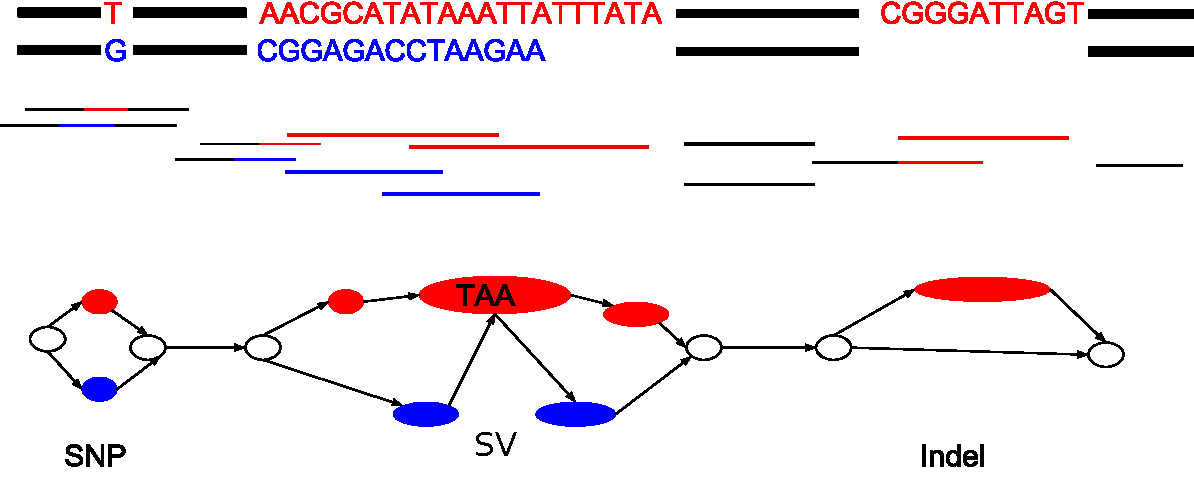
\includegraphics[width=\columnwidth]{ex_sv.pdf}
\caption{Based on reads (middle) from the two sequences (top), the bubbles in the graph (bottom) show three different heterozygous variations; the first one is an SNV, the second one is an SV, and the third one is an indel. }
\label{fig:ex_sv}
\end{figure}

\paragraph{De Bruijn graph and overlap graph}
The de Bruijn graph theoretically achieves
the same tasks that the overlap graph does, but in an efficient manner.
The de Bruijn graph became widely used when the short reads from NGS appeared. The OLC
approach did not scale well on the high number of sequences generated by NGS. The
use of the de Bruijn graph is very interesting for short read assembly for its ability to
deal with the high redundancy of such sequencing in a very efficient way. Indeed a kmer
present dozens of times in the sequencing dataset appears only once in the graph. This
makes the de Bruijn graph structure not very sensible to high coverage, unlike
OLC. The de Bruijn graph was first proposed as an alternative structure \citep{pevzner2001eulerian} because it
was less sensible to repeats. Repeats that were problematic in the OLC, creating very
complex and edges heavy zones, are collapsed in the de Bruijn graph.

\paragraph{Graph structures} There are mainly two types of structures that occur in the assembly graphs for diploid genomes.

\textit{Bubbles.}
Bubbles are defined as a set of disjoint paths that share the same start and end nodes.
Bubbles in the graph represent heterozygosity in the diploid organism.
Bubbles can contain simple SNVs with only one allele difference, or even large complex structural variations in the order of a few kilo-bases.  
Figure~\ref{fig:ex_sv} illustrates how the bubbles in an assembly graph can contain both small variants (SNPs and indels up to several dozen base-pairs in length) and larger structural variants.
\begin{figure}[t!]\centering
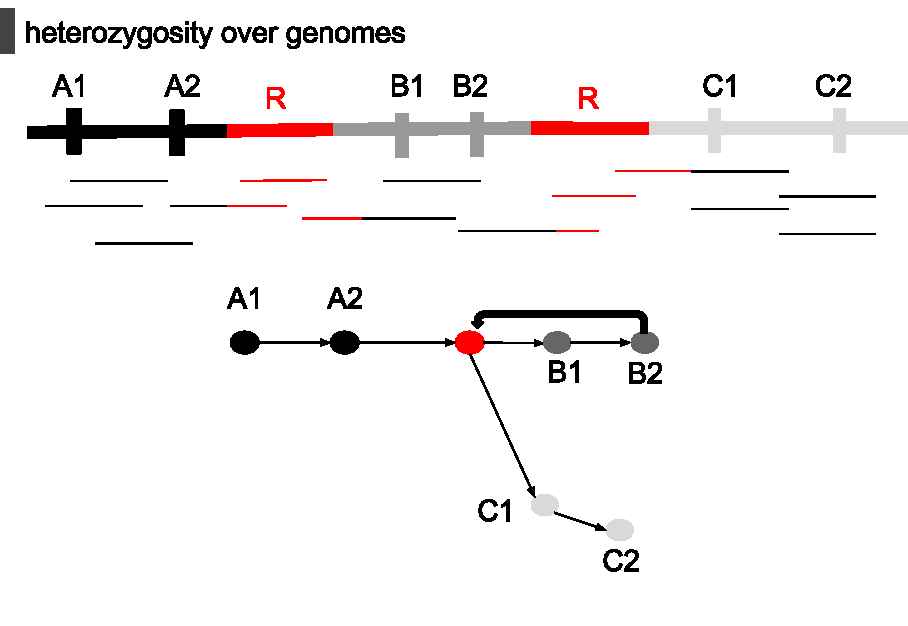
\includegraphics[width=\columnwidth]{repeats.pdf}
\caption{At the top, shown are the heterozygosity (in vertical bars) and repetitive regions (in red) over the genome. At the bottom, shown is the graph with nodes as heterozygous or repetitive region, and connections are based on the successive read overlap.
The graph has cycles because of repetitive region shown by R, which also causes two branches.}
\label{fig:repeats}
\end{figure}

\textit{Repeats.} The repeats over the genomes cause branches or cycles in the assembly graphs and, therefore, make a graph more complex and break its linear chain properties.
This is illustrated in Figure~\ref{fig:repeats}. In this example, the repeat $R$ causes cycles and branches in the graph.
Assemblers generally handle these repeats by making a guess as to which branch to follow.
Incorrect guesses create false joins (chimeric contigs) and erroneous copy numbers. 
If the assembler is more conservative, it will break the assembly at these branch points, leading to an accurate but fragmented assembly with fairly small contigs.
The maximal repeat resolution  depends on the read-length, if there is a read that is long enough to span the repeat region, then the repeat is resolvable.
Therefore, upcoming long-read sequencing technologies have the power to obtain maximal repeat-resolved haplotypes.

\subsection{Main approaches}
Over the last decade, the development of various NGS technologies has impacted the assembly problem.
In theory, the problem of \textit{de novo assembly}---computing the consensus of two or more sequences---is NP-hard, when the problem is modeled either as string graphs or de Bruijn graphs \citep{medvedev2007computability}. 
There are several heuristic approaches to approximate the optimal de novo haploid assembly based on NGS datasets \citep{idury1995new, myers1995toward, myers2005fragment, pevzner2001eulerian, nagarajan2009parametric, nagarajan2013sequence, sovic2013approaches}.

However, even with Sanger (reads of the order of 800-1000 base pairs) and Illumina sequencing, which deliver short reads with low error rates, de novo assembly of heterozygous diploid genomes has been a difficult problem \citep{vinson2005assembly, levy2007diploid}.
In practice, there are several short-read assemblers based on Illumina data for heterozygous genomes \citep{kajitani2014efficient, pryszcz2016redundans, simpson2012efficient, bankevich2012spades, li2015fermikit}.
The assemblies that they produce are accurate, but contain gaps and are composed of relatively short contigs and scaffolds. 
Third generation sequencing technologies such as methods available from Pacific Biosciences (PacBio) and Oxford Nanopore Technologies (ONT) deliver much longer reads, but with high error rates.
There are now several long-read assemblers \citep{koren2017canu, vaser2017fast, xiao2016mecat, berlin2015assembling, chin2013nonhybrid, hunt2015circlator, lin2016assembly} that use these long-read data for de novo assembly.
The assemblies that are delivered from these assemblers are more contiguous, with longer contigs and scaffolds.
Finally, there are hybrid assemblers that take advantage of long-read data (with its high error rate) and short-read data (with its low error rate) \citep{bashir2012hybrid, antipov2015hybridspades, zimin2017hybrid} and attempt to combine the best aspects of both.
These hybrid assemblers have the power to deliver highly accurate, repeat-resolved assemblies.

A recent and only available diploid assembly method --- Falcon Unzip \citep{chin2016phased} --- is purely PacBio based diploid assembler.
Falcon Unzip generates haplotype contigs or ``haplotigs'' that represent the diploid genome with correctly phased homologous chromosomes.
Falcon Unzip basically constructs a string graph from long PacBio reads, and then potentially finding haplotigs in a greedy manner using local conservative approach.
\begin{figure}[t!]\centering
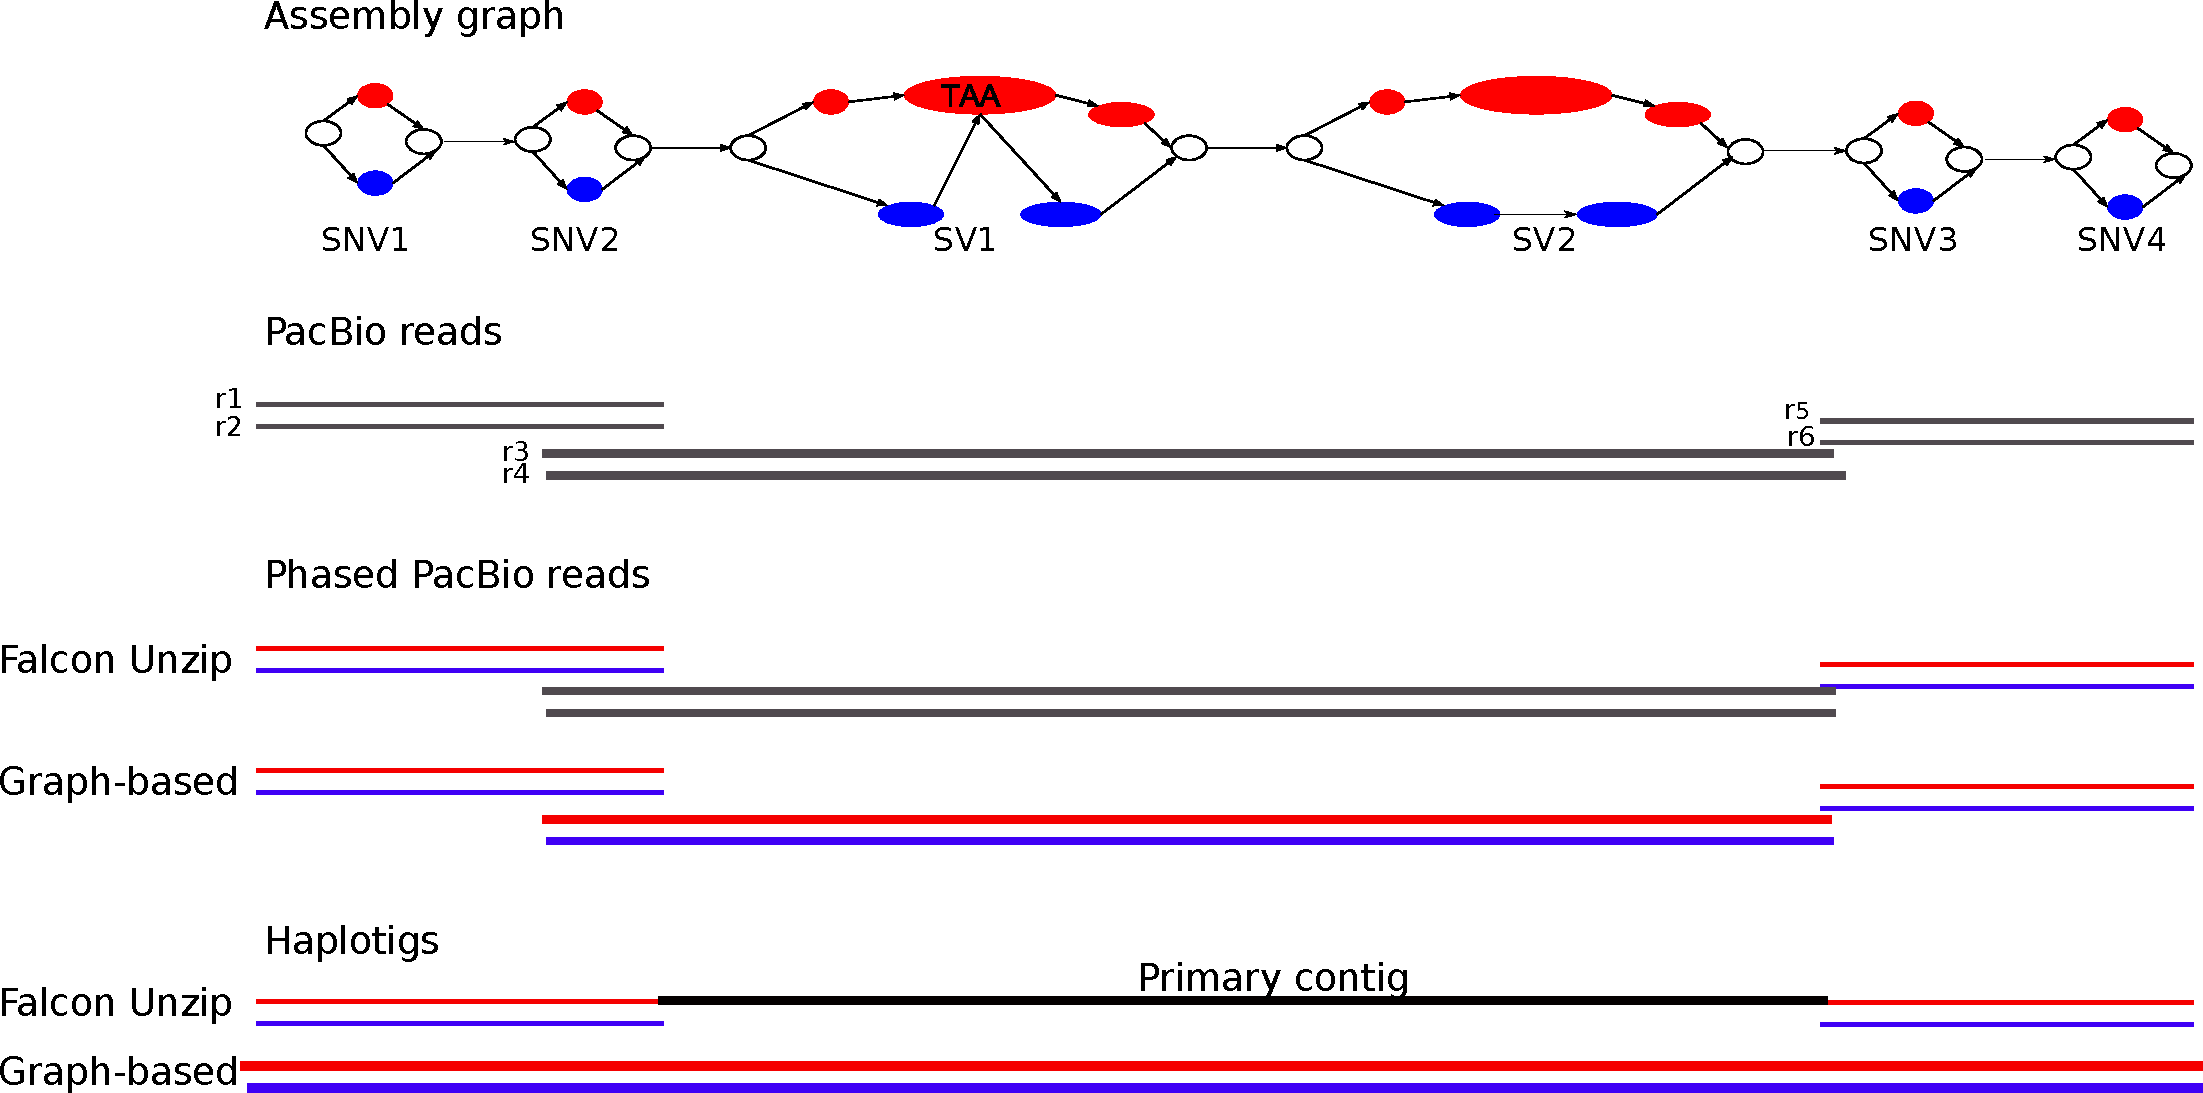
\includegraphics[width=\columnwidth]{ex_graph_approach.pdf}
\caption{Input: an assembly graph (top) (consisting of four SNVs and two SVs) and the PacBio reads $r_1, r_2, r_3, r_4, r_5, r_6$ (gray). 
Output: the phased reads (colored in blue and red) and haplotigs (bottom) using Falcon Unzip and our graph-based approach. Our graph-based phases central region, contrarily, Falcon Unzip does not.  }
\label{fig:ex_graph_approach}
\end{figure}

The main drawback of this approach is that it can not phase large structural variants. Additionally, Falcon Unzip requires that the PacBio read cover at-least one SNV for phasing.
In the situations where the SNVs are at a long distance to each other, the Falcon Unzip can not phase those regions, resulting in incomplete assemblies.
% The pipeline is given in Figure~\ref{fig:falcon_unzip}.
% Falcon Unzip begins by using reads to construct a string graph that contains sets of ``haplotype-fused contigs'' , also called as ``primary contigs'', as well as bubbles representing divergent regions between homologous sequences (Fig.~\ref{fig:falcon_unzip}a). 
% Next, Falcon-Unzip identifies read haplotypes using phasing information from heterozygous positions that it identifies (Fig.~\ref{fig:falcon_unzip}b). 
% Phased reads are then used to assemble haplotigs and primary contigs (backbone contigs for both haplotypes) (Fig.~\ref{fig:falcon_unzip}c) 
% that form the final diploid assembly with phased single-nucleotide polymorphisms (SNPs) and structural variants (SVs).
% 
% \textit{Phasing using primary contigs.}
% In Falcon Unzip, the reads are aligned to primary contigs and heterozygous SNPs (het-SNPs) are called by analyzing the base frequency of the detailed sequence alignments.
% A simple phasing algorithm was developed to identify phased SNPs. 
% Along each contig, the algorithm assigns phasing blocks where ``chained phased SNPs'' can be identified. 
% Within each block, if a raw read contains a sufficient number of het-SNPs, it assigns a haplotype phase for the read unambiguously. 
% Combined with the block and the haplotype phase information, it assigns a ``block-phase'' tag for each phased read in each phasing block.
% Some reads might not have enough phasing information. For example, if there are not enough het-SNP sites covered by a read, it assigns a special 'un-phased tag' for each un-phased read.
% The initial assembly graph is fused using phased reads and the haplotigs are generated in a greedy manner using local conservative approach.
% % \todo{maybe add example how haplotigs from haplotype fused assembly graph works?}

% \begin{figure}[t!]\centering
% \includegraphics[width=\columnwidth]{{cropped_falcon-unzip}.pdf}
% \caption{(a) An initial assembly is computed by FALCON, which error corrects the raw reads (not shown) and then assembles them using a string graph of the read overlaps. 
% The assembled contigs are further refined by FALCON-Unzip into a final set of contigs and haplotigs. 
% (b) Phase heterozygous SNPs and group reads by haplotype. (c) The phased reads are used to open up the haplotype-fused path and generate as output a set of primary contigs and associated haplotigs.}
% \label{fig:falcon_unzip}
% \end{figure}

A potential step to fix these problems is phasing directly from the assembly graph. 
In doing so, reads are aligned to the assembly graph and thus reads have a better chance to be more accurately aligned.
Moreover, it is easier to detect large structural variants, such as translocations and other rearrangements, in an assembly graph.
Thus, working in the space of assembly graphs provide deep insights to detect all types of structural variation, which further helps in phasing whole genomes.
\begin{gaps}
 Phasing bubbles directly from the assembly graph is an open problem. Additionally, finding MEC formulation for solving phasing using hybrid of multiple sequencing technologies, is unknown. 
 \label{gap:gap4}
\end{gaps}

\begin{example}
Figure~\ref{fig:ex_graph_approach} demonstrates the advantages of our graph-based approach over the Falcon Unzip method.
Consider four SNVs separated by two large SVs and there are four reads spanning these variants.
Falcon Unzip can not phase the central region because the reads $r_3$ and $r_4$ do not cover any SNVs, resulting in incomplete haplotigs.
In contrast, the graph-based approaches attempt to detect all types of SVs and phase all of them.
\end{example}
Based on the above example, we observe that it is possible to deliver more complete and contiguous haplotigs using our graph-based approach.

% \begin{figure}[t!]\centering
% 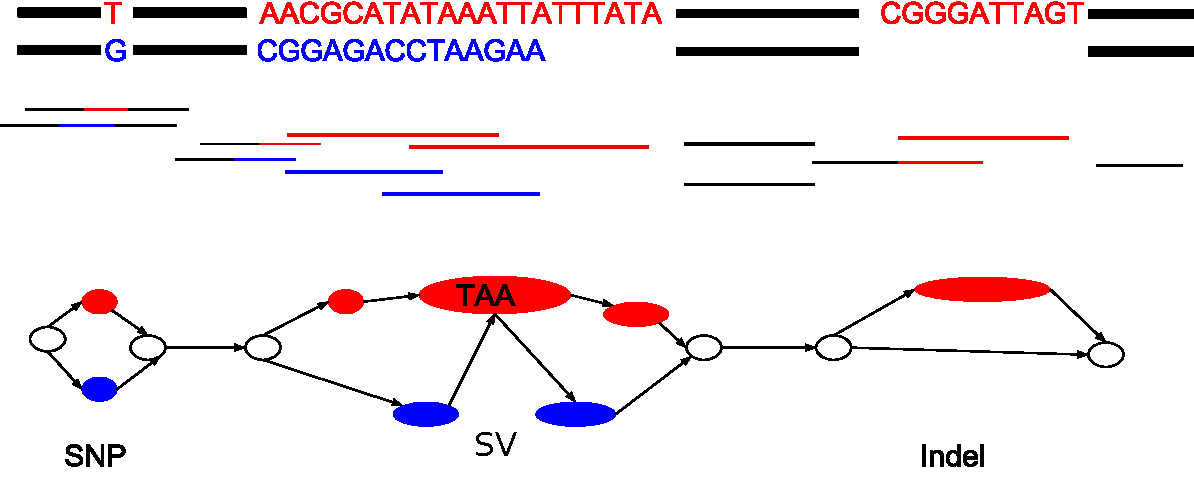
\includegraphics[width=\columnwidth]{ex_sv.pdf}
% \caption{Based on reads (middle) from the two sequences (top), the bubbles in the graph (bottom) show three different heterozygous structural variations; first is a SNV, second is a SV and third is an indel. }
% \label{fig:ex_sv}
% \end{figure}
\section{Outline of our contributions}
In the above section, I highlighted four ``open problems'' in the arena of haplotyping using NGS data.

\begin{itemize}
 \item In Chapter 2, I provide a general background on the different types of algorithms. I outline the motivation on how these algorithms are used in solving small daily examples fast. 
 I highlight the advantages and disadvantages of these algorithms in context of large problems.
 \item Solving MEC instances using NGS data are NP-hard. In Chapter 3, I describe the dynamic programming based algorithm to solve these instances approximately.
 I discuss the approximation guarantee, which provides hints that these instances can be solved in practice in polynomial time. (Problem~\ref{gap:gap1})
  \item In Chapter 4, I discuss different types of NGS datasets, with their advantages and disadvantages. I describe the integrative phasing framework obtained by combining NGS datasets. I discuss the parameterized algorithm that solves these instances efficiently in practice. 
  I demonstrate the effectiveness of this algorithm on real genomic datasets. (Problem~\ref{gap:gap2})
 \item In Chapter 5, I describe the generalized parameterized approach to incorporate information from pedigrees. I show the experiments on real datasets and highlight that pedigree data has an additional advantage in delivering better quality haplotypes. (Problem~\ref{gap:gap3})
 \item In Chapter 6, I describe the generalized approach --- haplotype-aware diploid assembly --- in a graph framework, that has the ability to handle all levels of heterozygosity and structural variations to produce accurate and complete haplotype assemblies.
 I present this approach as a hybrid of different types of NGS datasets and show its effectiveness on the real genome. (Problem~\ref{gap:gap4})
 \item Finally, in Chapter 7, I provide a summary of the results presented in this thesis, along with the future outlook and perspectives.
\end{itemize}

\section{Relationship to publications}
\begin{itemize}
 \item David Porubsky*, Shilpa Garg*, Ashley D. Sanders*, V. Guryev, Peter M. Lansdorp, T. Marschall,
\textit{Dense And Accurate Whole-Chromosome Haplotyping Of Individual Genomes}, Nature Communications, 2017.

In this paper, my contribution was in developing an integrative pipeline and writing draft for WhatsHap section.
\item Shilpa Garg, Marcel Martin and Tobias Marschall, \textit{Read-Based Phasing of Related Individuals},
Proceedings of ISMB 2016/Bioinformatics.
\item Shilpa Garg, Mikko Rautiainen, Adam M Novak, Richard Durbin, Tobias Marschall, \textit{A graph-based approach to diploid genome assembly}, Submitted.
\item Shilpa Garg, Tobias Moemke, \textit{A QPTAS for Gapless-MEC}, Submitted.
\item Preprint: M. Martin*, M. Patterson*, Shilpa Garg, S. O. Fischer, N. Pisanti, G. W. Klau, A. Schnhuth, T.
Marschall, \textit{WhatsHap: fast and accurate read-based phasing}.

In this paper, my contribution was in developing some parts of the pipeline and making initial figures.
\end{itemize}


% \subsection{Issues we address}
% To address those problems, we will present new algorithmic approaches. 
% \begin{itemize}
% \item In the second chapter, we present the fundamental concepts of different type of algorithms.
%  \item In the third chapter, we present dynamic programming based algorithm to prove the near-polynomial approximation status of \GMEC.
%  \item In the forth chapter, we present a parameterized algorithm to solve \MEC instances integatively from different datasets.
%   \item In the fifth chapter, we present a integrative framework to solve sequencing-based and genetic haplotyping, helps to generate complete and accurate haplotypes.
%  \item In the sixth chapter, we introduce new way to represent the assembly graph and futher, finding long read paths in the graph based on different types of datasets, which futher helps in better phasing. 
% \end{itemize}


% 
% 
%  
% 
% \todo{cover these issues in approaches}
% \subsection{Diploid genome assembly hardness}
% \begin{itemize}
% \item Theoretical approximation gurantee on gapless-MEC. It is important because even for high coverages, we can solve it in polynomial time approximately.
%  \item integrating datasets to produce more accurarte and complete
%  \item non-reference denovo based, can not detect large SVs, directly from graph, hybrid
%  \item pedigree of genomes
% \end{itemize}
% 
% \subsection{Goals and achievements}
% \begin{enumerate}
%  \item DNA genomes ranging from small yeast like genome to larger ones like human.
%  \item end-to-end full genome sequences
%  \item efficient algorithms to generate optimal or near-optimal solution.
% \end{enumerate}
% 
% 
% 
% 
% \subsection{Outline of our contributions}
% \begin{enumerate}
%  \item Chpater 1 consists of ...
%   \item Chpater 2 consists of ...
%    \item Chpater 3 consists of ...
% \end{enumerate}






